\documentclass[11pt,a4paper]{article}

% --- Packages ---
\usepackage[utf8]{inputenc}
\usepackage[english]{babel}
\usepackage[T1]{fontenc}
\usepackage{lmodern}
\usepackage{geometry}
\geometry{left=2cm, right=2cm, top=2cm, bottom=2cm}
\usepackage{enumitem}
\usepackage{titlesec}
\usepackage{hyperref}
\usepackage{xcolor}
\usepackage{tabularx}
\usepackage{graphicx}

% --- Color Definitions ---
\definecolor{color0}{rgb}{0,0,0}         % Main text color (Black)
\definecolor{color1}{RGB}{0, 75, 135}    % Academic Blue
\definecolor{color2}{gray}{0.3}          % Secondary info color

% --- Section Styling ---
\titleformat{\section}
  {\Large\bfseries\color{color1}}
  {}{0em}{}
  [\titlerule]
\titlespacing{\section}{0pt}{18pt}{10pt}

% --- Hyperref Setup ---
\hypersetup{
    colorlinks=true,
    linkcolor=color1,
    urlcolor=color1,
    pdftitle={Davide Chirichella - Curriculum Vitae},
}

% --- Custom Entry Commands ---
\newcommand{\cvitem}[2]{
    \noindent
    \begin{tabularx}{\textwidth}{@{}p{3.5cm} X@{}}
        \textbf{#1} & #2
    \end{tabularx}
    \vspace{4pt}
}

\newcommand{\cventry}[6]{
    \noindent
    \begin{tabularx}{\textwidth}{@{}p{3.5cm} X@{}}
        {\small\sffamily #1} & \textbf{#2} \\
        & \textit{#3}, #4 \\
        & \small #6
    \end{tabularx}
    \vspace{6pt}
}

\begin{document}

\pagestyle{empty}

% --- Header ---
\noindent
\begin{minipage}[t]{0.75\textwidth}
    \raggedright
    {\Huge \textbf{Davide Chirichella}} \\
    \vspace{2mm}
    {\large \textcolor{color1}{Computer Engineering Master's Student | Academic Tutor | Developer}}
\end{minipage}
\begin{minipage}[t]{0.25\textwidth}
    \raggedleft
    \vspace{-4mm}
    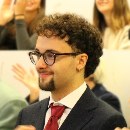
\includegraphics[width=2.8cm]{picture.png}
\end{minipage}

\vspace{6mm}

\section{Personal Information}
\cvitem{Full Name}{Davide Chirichella}
\cvitem{Date of Birth}{November 10th, 2003}
\cvitem{Citizenship}{Italian}
\cvitem{Current Location}{Bologna, Italy}
\cvitem{Email}{\href{mailto:davidechirichella10@gmail.com}{davidechirichella10@gmail.com}}
\cvitem{LinkedIn}{\href{https://www.linkedin.com/in/davide-chirichella-88200b1ba/}{linkedin.com/in/davide-chirichella}}
\cvitem{GitHub}{\href{https://github.com/chirichexe}{github.com/chirichexe}}

\section{Profile}
\noindent Master's student in \textbf{Computer Engineering} at the University of Bologna and \textbf{Academic Tutor} for System Administration. Specializing in the design and management of \textbf{distributed systems} and \textbf{microservices architectures}, with a core interest in building scalable, reliable, and resilient systems. Strong background in software development, DevOps, and cloud-edge computing.

\section{Education}
\cventry{2025 -- Present}{Master's Degree in Computer Engineering}{Alma Mater Studiorum --- Università di Bologna}{Bologna}{}{Focus on Distributed Systems, CUDA parallel computing, and Go-based systems.}

\cventry{2022 -- 2025}{Bachelor's Degree in Computer Engineering}{Alma Mater Studiorum --- Università di Bologna}{Bologna}{Grade: 107/110}{
\begin{itemize}[noitemsep, topsep=0pt, leftmargin=1em]
    \item \textbf{Thesis:} ``Performance Analysis and Monitoring in Cloud-Edge environments for IoT''
    \item \textbf{Project KOPIC:} Developed a distributed architecture for orchestrating low-power IoT devices across the cloud-edge continuum using Kubernetes Operators, Crossplane, and a full observability stack (Prometheus, Grafana, OpenTelemetry).
    \item Curricular internship (150 hours) at the Department of Computer Science and Engineering (DISI).
\end{itemize}}

\cventry{2017 -- 2022}{High School Diploma}{Liceo Scientifico Galileo Galilei}{Potenza}{}{Focus on Adobe Creative Cloud, Multimedia Content Production, and Graphic Design.}

\section{Experience}
\cventry{Feb 2026 -- Pres}{Academic Tutor (System Administration)}{Alma Mater Studiorum --- Università di Bologna}{Bologna}{}{
\begin{itemize}[noitemsep, topsep=0pt, leftmargin=1em]
    \item Supporting the course ``System Administration and Security'' for undergraduate students.
    \item Instruction in Linux administration, security auditing, and automation.
\end{itemize}}

\cventry{Feb 2026 -- Pres}{Junior DevOps Engineer}{HoDiritto (Startup)}{Remote}{}{
\begin{itemize}[noitemsep, topsep=0pt, leftmargin=1em]
    \item Built and managed infrastructure, CI/CD, and monitoring for an early-stage MVP within a pre-acceleration program.
    \item Technologies: Microservices, Terraform, Docker, and Kubernetes.
\end{itemize}}

\cventry{2023 -- 2026}{Software Engineer / Developer}{Project Quality Systems S.R.L.}{Remote}{}{
\begin{itemize}[noitemsep, topsep=0pt, leftmargin=1em]
    \item Designed and developed a C\# desktop application for company audits.
    \item Full-stack development of the corporate management system using React.js, Node.js, and MySQL.
\end{itemize}}

\section{Technical Skills}
\cvitem{Languages}{Go, CUDA, C, Java, C\#, JavaScript (React.js, Node.js), SQL, Python.}
\cvitem{Cloud/DevOps}{Kubernetes, Docker, Terraform, CI/CD, Istio, Crossplane.}
\cvitem{Observability}{Prometheus, Grafana, OpenTelemetry.}
\cvitem{Systems}{Linux System Administration, Shell Scripting, Cybersecurity basics.}
\cvitem{Tools}{Git, Adobe Creative Suite (Photoshop, Illustrator, Premiere).}

\section{Languages \& Honors}
\cvitem{English}{Cambridge English First (FCE) --- Level B2.}
\cvitem{Italian}{Native speaker.}
\cvitem{Projects}{Contributor to various open-source distributed systems and DevOps projects on GitHub.}

\end{document}
